\documentclass[a4paper]{article}

\usepackage{caption}
\usepackage{listings}
\usepackage{fancyhdr}
\usepackage[top=3cm,bottom=3cm,left=3cm,right=3cm]{geometry}
\usepackage{color}
\usepackage{amsmath}
\usepackage{graphicx}
\usepackage{tabulary}

\definecolor{dkgreen}{rgb}{0,0.6,0}
\definecolor{gray}{rgb}{0.5,0.5,0.5}
\definecolor{mauve}{rgb}{0.58,0,0.82}

\lstset{frame=tb,
  language=Octave,
  aboveskip=3mm,
  belowskip=3mm,
  showstringspaces=false,
  columns=flexible,
  basicstyle={\small\ttfamily},
  numbers=none,
  numberstyle=\tiny\color{gray},
  keywordstyle=\color{blue},
  commentstyle=\color{dkgreen},
  stringstyle=\color{mauve},
  breaklines=true,
  breakatwhitespace=true,
  tabsize=3
}

\newcommand{\HRule}{\rule{\linewidth}{0.5mm}}
\pagestyle{fancy}
\lfoot{\small \color{gray}Tom Peerdeman - 10266186}
\cfoot{\thepage}
\rfoot{\small \color{gray}Ren\'e Aparicio Sa\'ez - 10214054}
\lhead{\small \color{gray}Autonome Mobiele Robots}

\begin{document}
\begin{titlepage}
\begin{center}
\textsc{\Large Autonome Mobiele Robots}\\[0.5cm]
\HRule \\[0,4cm]
\textsc{\huge \bfseries NXT - Localisering door middel van lijnen en blobs}
\HRule \\[8cm]
\begin{minipage}{0.4\textwidth}
\begin{flushleft}\large
\emph{Auteurs: Tom Peerdeman \& Ren\'e Aparicio Saez}\\
\end{flushleft}
\end{minipage}
\begin{minipage}{0.4\textwidth}
\begin{flushright}\large
\emph{Datum: \today\\\hspace{1cm}}\\
\end{flushright}
\end{minipage}
\end{center}
\end{titlepage}

\tableofcontents
\newpage

\section{Materiaal}
Om de experimenten uit dit rapport te kunnen uitvoeren zijn de volgende materialen gebruikt:\\
- PC/Laptop met Matlab\\
- Boek: Autonomous Mobile Robots 2th Edition - Roland Siegwart et al.\\
- NXT-Robot\\
- Logitech Webcam\\
- Gloeilamp\\
- Zwarte tape

\section{Introduction}
Een autonome mobiele robot moet weten waar in de wereld hij momenteel is. Als er een kaart bekend is kan aan de hand van de omgeving die de robot momenteel detecteert bepaald worden waar in de wereld hij is. Dit kan gedaan worden aan de hand van de detectie van lijnen en blobs in zijn huidige omgeving en deze te vergelijken met de bekende blobs die opgeslagen zijn in de kaart. Gecombineerd zullen de lijnen en blobs een goede indicatie kunnen geven over de locatie van de robot.

\section{Fouten in meegeleverde code}
De meegeleverde code bevatte enkele fouten. Zo was het omzetten van het opgenomen beeld naar een zwart wit beeld 'geinverteerd' (zwart was wit en andersom). 
Tevens was het bestand imflipud.m aangepast. Het bestand imflipud.m zou een functie moeten leveren om een plaatje verticaal te spiegelen om zijn middelpunt. Het gegeven bestand bevatte echter een functie die helemaal niks deed met het plaatje.\\


\section{Maken van een dataset}
\subsection{Foto's maken}
Om experimenten uit te kunnen voeren is een dataset nodig. Deze dataset moet bestaan uit fotos die een afgeplakt parcour volledig omschrijven. Er moet hiervoor een parcour gemaakt worden met behulp van tape. Vervolgens moeten er voldoende fotos gemaakt worden zodat het gehele parcour gezien wordt. Voor de experimenten is het ook nodig dat het parcour gesloten is. Na het maken van de eerste dataset bleek er echter geen rekening gehouden te zijn met het maken van een tweede testset. Er moet opnieuw een dataset gemaakt worden op een nieuw parcour (het oude parcour is al weggegooid). Dit nieuwe parcour wordt gebruikt voor zowel de train-set als de test-set. In figuur \ref{fig:datasetmaken} is te zien hoe er te werk is gegaan bij het maken van een dataset. In figuur \ref{fig:plattegrond} is te zien hoe de uiteindelijke plattegrond van de dataset er uit is komen te zien.
\begin{figure}[h]
	\centering
	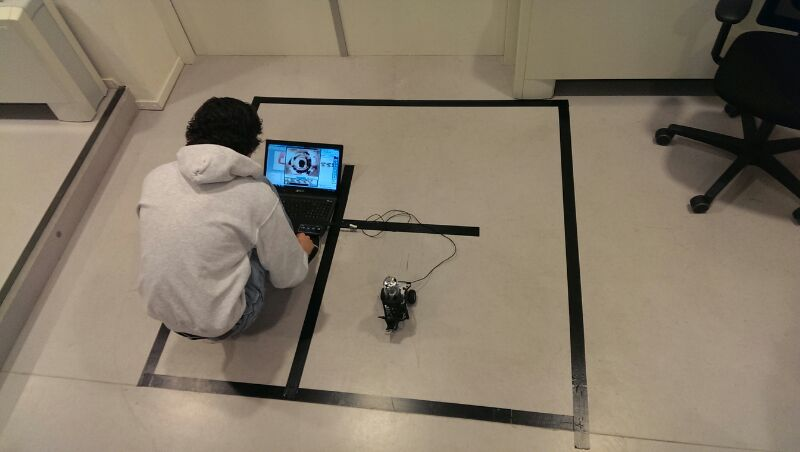
\includegraphics[width=0.7\textwidth]{dataset1.jpg}
	\caption{Het maken van een dataset (niet gebruikte dataset)}
	\label{fig:datasetmaken}
\end{figure}
\begin{figure}[h]
	\centering
	\includegraphics[width=0.8\textwidth]{opzet.png}
	\caption{Plattegrond en locaties van de gemaakte fotos}
	\label{fig:plattegrond}
\end{figure}

\subsection{Parameters}
De parameters moeten worden aangepast aan de nieuwe dataset. De camera is lichtelijk verschoven en moest verstevigd worden waardoor de positie van de lamp en het middelpunt van de camera is verplaatst ten op zichte van de vorige proeven. Het middelpunt heeft de coordinaten $x = 545$, $y = 402$. De radius blijft hetzelfde. Er zijn nog enkele uitwendige niet gebruikte sensoren van de robot afgehaald waardoor de waarden voor Rmin kan worden verlaagd. De waarde wordt verlaagd naar Rmin $= 115$. De waarde voor Rmax wordt aangepast vanwege de verplaatste locatie van de bolling ten opzichte van de camera. De waarde van Rmax wordt: Rmax $= 190$. De waarde van $\alpha$ wordt geschat door te kijken naar de manier waarop het gemeten beeld wordt 'rechtgetrokken'. De waarde veranderd naar $\alpha = 140$. Tot slot wordt de treshold voor de zwart-wit beelden aangepast. Dit wordt gedaan omdat de nieuwe opnamen geen verhoogd contrast hebben (dit was bij de vorige dataset wel het geval). De nieuwe waarde wordt  $treshold = 130$.


\section{Line fingerprints}
Met behulp van de code uit het vorige labexperiment kunnen lijnen worden gedetecteerd. Met behulp van deze code kunnen deze gevonden lijnsegmenten worden opgebouwd. Dit wordt gedaan met een meegeleverd 'split \& merge' algoritme. De gecombineerde lijnsegmenten in een foto vormen een fingerprint voor de lijnen op die locatie. In figuur \ref{fig:lijnfinger} is zo een fingerprint te zien. 
In figuur \ref{fig:confusion_line} is te zien hoe uniek deze fingerprints zijn. Als de fingerprints namelijk veel overeenkomen, dan is de Levenshtein afstand tussen deze fingerprints ook laag. Indien de Levenshtein afstand laag is zal het moeilijker worden om een duidelijke locatie aan te geven omdat de kans dat de robot dan op de ene locatie is heel erg dicht bij de kans voor een andere locatie liggen kan. 
Als de robot vervolgens de testset bekijkt, worden de fingerprints die opgebouwd worden voor de test-set vergeleken met de fingerprints van de train-set. Hieruit kan de waarschijnlijkheid bepaald worden voor de huidige locatie van de robot. Dit kan worden weergegeven in een matrix, zoals te zien is in figuur \ref{fig:line_prob}

\begin{figure}[h]
	\centering
	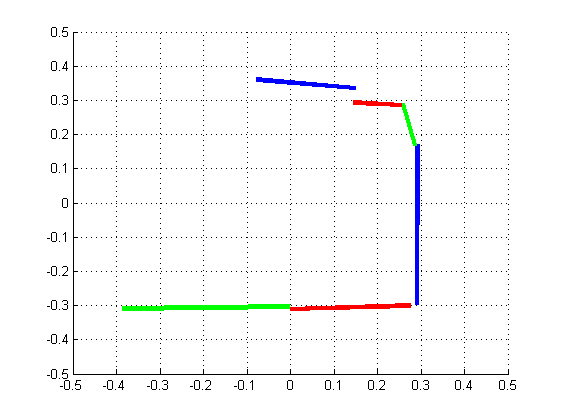
\includegraphics[width=0.8\textwidth]{fingerprint.png}
	\caption{Fingerprint voor lijnsegmenten}
	\label{fig:lijnfinger}
\end{figure}


\section{Blob fingerprints}
Met behulp van meegeleverde code wordt gezocht naar blobs. Er moet echter aangegeven worden naar welke kleurwaarden er gekeken moet worden. Aangezien er geen kleuren in het parcour zijn verwerkt moet dit worden aangepast. Door dit aan te passen zodat er alleen een onderscheidt wordt gemaakt tussen zwart en wit wordt dit overkomen. In de originele code wordt gekeken naar twee kleuren. Er wordt dan een blob gedetecteerd als er een blob in een van de twee kleuren voorkomt.  Aangezien de aangepaste versie niet meer gebruikt maakt van kleur is de detectie van de tweede kleur compleet verwijderd. 
De combinatie van de blobs in een beeld vormt een fingerprint, een voorbeeld is te zien in figuur \ref{fig:blobfinger}. In dit figuur staan een heleboel blobs, echter word net als bij de lijn alleen de blobs gebruikt die tussen Rmin en Rmax vallen. 
De confusion matrix voor blobs is weergegegeven in figuur \ref{fig:confusion_blob}.
Bij het testen moet er worden gezocht naar een match tussen de bekende fingerprints en de huidige gemeten set blobs. Er kan weer een waarschijnlijkheid worden bepaald voor de locatie van de robot en deze kan worden weergegeven met behulp van een matrix (figuur \ref{fig:blob_prob}).

\begin{figure}[h]
	\centering
	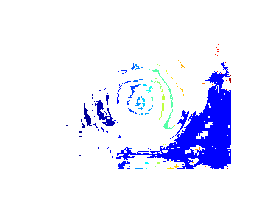
\includegraphics[width=0.7\textwidth]{fingerprintblob.png}
	\caption{Fingerprint voor blobs}
	\label{fig:blobfinger}
\end{figure}


\section{Gecombineerde fingerprints}
\subsection{Gewogen fingerprints}
De eerste manier om de fingerprints te combineren is aan de hand van het toekennen van gewichten. Door een gewicht toe te kennen voor de fingerprint van de lijnsegmenten en een tweede gewicht toe te kennen aan de fingerprint van de blobs kan aangegeven worden welk van de twee zwaarder meetelt. Het gewicht voor de lijnsegmenten wordt vermenigvuldigt met de gevonden waarschijnlijkheid voor die specifieke fingerprint. Ditzelfde wordt gedaan voor de blobs en deze gewogen waarden worden bij elkaar opgeteld. Vervolgens kan aan de hand van de confusion matrix bekeken worden wat de waaarschijnlijkheid is op een locatie te zijn als gebruik is gemaakt van deze gecombineerde methode. De waarschijnlijkheids matrix is zichtbaar in figuur \ref{fig:combinedconfusion}.

\subsection{Geconcateneerde fingerprints}
Een tweede manier om de fingerprints te combineren is door de fingerprints te concateneren. De gevonden lijnsegmenten fingerprint en de blob fingerprint voor de train-set worden geconcateneerd en vervolgens vergeleken met de geconcateneerde fingerprint voor de lijnsegmenten die momenteel worden gezien en de fingerprint van de blobs die momenteel worden waargenomen. Hieruit volgt een confusionmatrix die een waarschijnlijkheid opleverd. De waarschijnlijkheids matrix is zichtbaar in figuur \ref{fig:combinedconfusion_concat}.

\section{Line segment lengths}
Aangezien de code niet rotatie invariant is, moet hier een oplossing voor worden gevonden. Een mogelijkheid is het bekijken van de lengte van de lijnsegmenten. Door deze lengtes van de lijnsegmenten in de fingerprint op te slaan en deze te vergelijken met de lengte van gemeten lijnsegmenten kan een vorm van rotatieinvariantie worden bereikt. Om ruis en error te voorkomen wordt gebruik gemaakt van een bereik van lengtes. Lengtes kunnen immers op een foutieve manier worden berekend. De matrix voor de resultaten is te zien in figuur \ref{fig:linelength}.

\section{Resultaten}
In tabel \ref{tab:normal} en tabel \ref{tab:combo} is te zien bij welk plaatje uit de train-set de robot hoort te zijn ten op zichte van het plaatje uit de test-set. Daarnaast staat in de tabel aangegeven waar de robot denkt te zijn aan de hand van de verschillende methoden.
\begin{table}[h]
  \centering
  \begin{tabulary}{\textwidth}{| C | C | C | C |}
    \hline
    Test-set \newline nummer & Train-set \newline nummer &  Lijnsegment fingerprint \newline location &  Blob fingerprint \newline location\\ \hline
    1 & 7 of 8 & 3 of 5 & 8\\ \hline
    2 & 7 of 8 & 7 & 1\\ \hline
    3 & 4 of 5 & 5 & 6\\ \hline
    4 & 2 & 3 & 3 of 4\\\hline
    5 & 8 & 3 &  6 \\\hline
    6 & 8 & 2 of 4 & 1 of 6\\ \hline
    7 & 6 of 7 & 8 & 8\\ \hline
    8 & 1 of 2 & 1 & 4 of 8\\ \hline
  \end{tabulary}
  \caption{Resultaten losse localisering}
  \label{tab:normal}
\end{table}
\newpage
\begin{table}[h]
  \centering
  \begin{tabulary}{\textwidth}{| C | C | C | C |}
    \hline
    Test-set \newline nummer & Train-set  \newline nummer &  Gewogen fingerprints location \newline gewicht line = 0.5; gewicht blob = 1 &  Geconcateneerde fingerprints \newline location\\ \hline
    1 & 7 of 8 &  8 & 8\\ \hline
    2 & 7 of 8 &  7 & 1 of 7\\ \hline
    3 & 4 of 5 &  6& 6\\ \hline
    4 & 2 &  3 & 3\\ \hline
    5 & 8 &  3 & 3  \\ \hline
    6 & 8 & 8 & 8\\ \hline
    7 & 6 of 7 & 8 & 8 \\ \hline
    8 & 1 of 2 & 4 of 8 & 8\\ \hline
  \end{tabulary}
  \caption{Resultaten gecombineerde localisering}
  \label{tab:combo}
\end{table}
\hspace{-0.68cm}
De gecombineerde gewogen fingerprints methode is de beste methode met een correcte evaluatie van ongeveer 40 tot 65 \% (slechts 3 van de 8 volledig goed, maar ook enkele bijna goed). Dit komt doordat de errors van beide fingerprints worden geconvolueerd en deze hierdoor een kleinere error opleveren. Door een juist gewicht uit te zoeken kan dit verder beinvloed worden om een goed resultaat te vinden.
\begin{table}[h]
  \centering
  \begin{tabulary}{\textwidth}{| C | C | C |}
    \hline
    Test-set \newline nummer & Train-set  \newline nummer & Line-length locatie \\ \hline
    1 & 7 of 8 &  1 \\ \hline
    2 & 7 of 8 &  7 of 8\\ \hline
    3 & 4 of 5 &  7\\ \hline
    4 & 2 &  1 \\ \hline
    5 & 8 &  4 \\ \hline
    6 & 8 &  8 \\ \hline
    7 & 6 of 7 & 1 \\ \hline
    8 & 1 of 2 & 7\\ \hline
  \end{tabulary}
  \caption{Resultaten line-length localisering}
  \label{tab:linelength}
\end{table}

\hspace{-0.68cm}
De localisering met behulp van de line-length werkt niet goed. Dit kan te maken hebben met een foute implementatie of verkeerde parameters waardoor lengtes van lijnen niet even lang zijn in verschillende locaties in het beeld.

\section{Verbeteringen}
Momenteel worden blobs gedetecteerd die niet per se altijd in de wereld aanwezig zijn. Denk aan mensen die in de train-set als blob zijn gedetecteerd, die hoeven niet de hele tijd op dezelfde locatie te blijven staan. Daarnaast zijn de lijnen allemaal zwart. Als elke lijn een eigen kleur had gekregen had de blobdetectie waarschijnlijk beter gewerkt.\\
Daarnaast is het algoritme niet rotatie invariant. Dit zorgt ervoor dat de gebruikte train en test set geen extreem hoge nauwkeurigheid oplevert. Er kan bijvoorbeeld gebruik gemaakt worden van SIFT in combinatie met een algoritme als RANSAC om dit wel te bewerkstelligen. Dit zal de nauwkeurigheid verbeteren.

\section{Code Snippets}
Hieronder zijn enkele code snippets te vinden van nieuw geschreven code.\\\\
De file Checkpattern is geschreven om een confusionmatrix op te stellen voor het vergelijken van een aangegeven gelabelde set metingen en een aangegeven ungelabelde set matingen.
\begin{lstlisting}[caption= CheckPattern.m, label=lst:checkpattern, numbers=left]
function confusion = CheckPattern(TrainFile, TestFile)
load(TrainFile);

PatStringsTrain = PatStrings;

load(TestFile);

st = size(PatStringsTrain, 2);   
sz = size(PatStrings, 2);
confusion = zeros(st, sz);

for i = 1:st
	for j = 1:sz
        lt = length(PatStringsTrain{i});
	    confusion(j,i) = ((lt - LevenshteinDistance(PatStringsTrain{i}, PatStrings{j})) / lt) * 100;
	end
end

% plot confusion matrix
colormap('gray')
imagesc(confusion);
\end{lstlisting}
De file CheckPatternCombined is geschreven om een confusionmatrix op te stellen voor het vergelijken van de gewogen gecombineerde methode. Hierbij moeten de gewichten aan de functie wordenmeegegeven.

\begin{lstlisting}[caption= CheckPatternCombined.m, label=lst:checkcombined, numbers=left]
function confusion = CheckPatternCombined(wline, wblob)
load 'LabeledLineSignatures.mat';
PatStringsLine = PatStrings;

load 'LabeledBlobSignatures.mat';
PatStringsBlob = PatStrings;

load 'UnlabeledLineSignatures.mat';
PatStringsUnLine = PatStrings;

load 'UnlabaledBlobSignatures.mat';
PatStringsUnBlob = PatStrings;

st = size(PatStringsLine, 2);   
sz = size(PatStringsUnLine, 2);
confusion = zeros(st, sz);

for i = 1:st
	for j = 1:sz
        ltl = length(PatStringsLine{i});
        ltb = length(PatStringsBlob{i});
        q1 = ((ltl - LevenshteinDistance(PatStringsLine{i}, PatStringsUnLine{j})) / ltl) * 100;
        q2 = ((ltb - LevenshteinDistance(PatStringsBlob{i}, PatStringsUnBlob{j})) / ltb) * 100;
        confusion(j,i) = wline * q1 + wblob * q2;
	end
end

% plot confusion matrix
colormap('gray')
imagesc(confusion);
\end{lstlisting}
De file CheckPatternCombined is geschreven om een confusionmatrix op te stellen voor het vergelijken van de geconcateneerde gecombineerde methode.

\begin{lstlisting}[caption= CombineSignatures.m, label=lst:checkconcat, numbers=left]
load 'LabeledLineSignatures.mat';
PatStringsLine = PatStrings;

load 'LabeledBlobSignatures.mat';
PatStringsBlob = PatStrings;

load 'UnlabeledLineSignatures.mat';
PatStringsUnLine = PatStrings;

load 'UnlabaledBlobSignatures.mat';
PatStringsUnBlob = PatStrings;

npatterns = size(PatStringsLine, 2);

PatStrings = [];
PatStringsUn = [];

for i=1:npatterns
    PatStrings{i} = [PatStringsLine{i} PatStringsBlob{i}];
    PatStringsUn{i} = [PatStringsUnLine{i} PatStringsUnBlob{i}];
end

save 'LabeledSignatures.mat' PatStrings PlaceID;

PatStrings = PatStringsUn;
save 'UnlabeledSignatures.mat' PatStrings;

\end{lstlisting}
Code om de line lengths mee te bepalen voor rotatie invariantie.
\begin{lstlisting}[caption= ComputePatStringLineLengths.m, label=lst:checkconcat, numbers=left]
% this function computes the pattern string based on the extracted segments
% and openings. The input segments are in a sequence. 
function  S = ComputePatStringLineLengths(NLines, ~, seglen, multiplier)
S = [];

j = 1;
for q=1:10
    bins(j:(j + 25)) = q;
    j = j + 25;
end


for i=1:NLines
    S = [S, bins(round(seglen(i)*multiplier))];
end

S

return
\end{lstlisting}


\section{Probability \& Confusion matrices}

\begin{figure}[h]
	\centering
	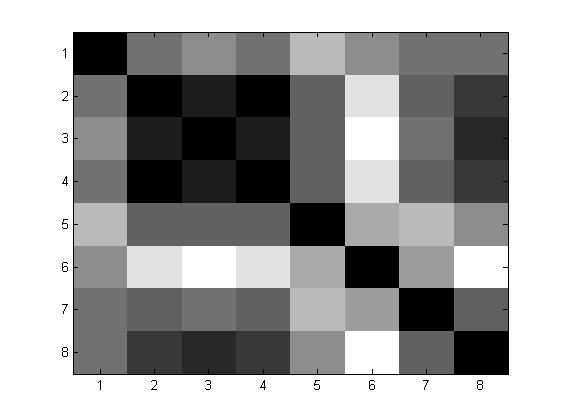
\includegraphics[width=0.8\textwidth]{confusion_line.jpg}
	\caption{Confusion matrix voor lijnsegmenten. Hoe lichter het vakje des te groter de Levenshtein distance.}
	\label{fig:confusion_line}
\end{figure}

\begin{figure}[h]
	\centering
	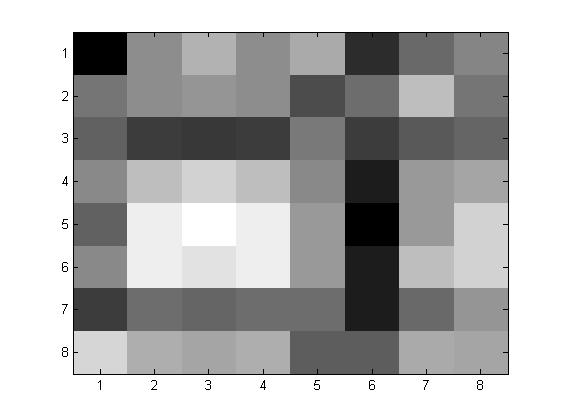
\includegraphics[width=0.8\textwidth]{line_prob.jpg}
	\caption{Waarschijnlijkheids matrix voor lijnsegmenten. Op de x as de test locaties en op de y as de train locaties. Hoe lichter het vakje des te groter de berekende kans.}
	\label{fig:line_prob}
\end{figure}

\begin{figure}[h]
	\centering
	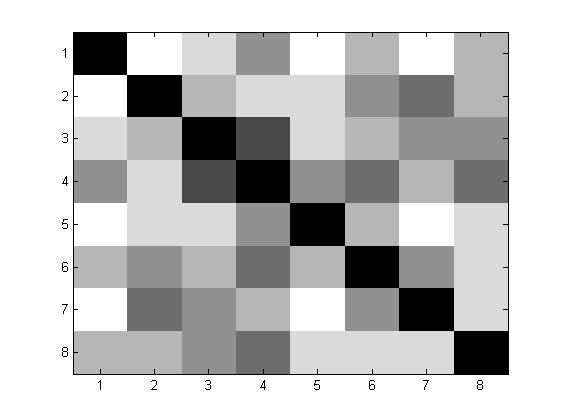
\includegraphics[width=0.8\textwidth]{confusion_blob.jpg}
	\caption{Confusion matrix voor blobs. Hoe lichter het vakje des te groter de Levenshtein distance.}
	\label{fig:confusion_blob}
\end{figure}

\begin{figure}[h]
	\centering
	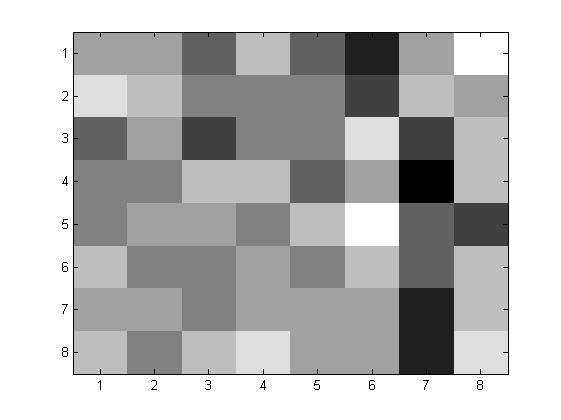
\includegraphics[width=0.8\textwidth]{blob_prob.jpg}
	\caption{Waarschijnlijkheids matrix voor blobs. Op de x as de test locaties en op de y as de train locaties. Hoe lichter het vakje des te groter de berekende kans.}
	\label{fig:blob_prob}
\end{figure}

\begin{figure}[h]
	\centering
	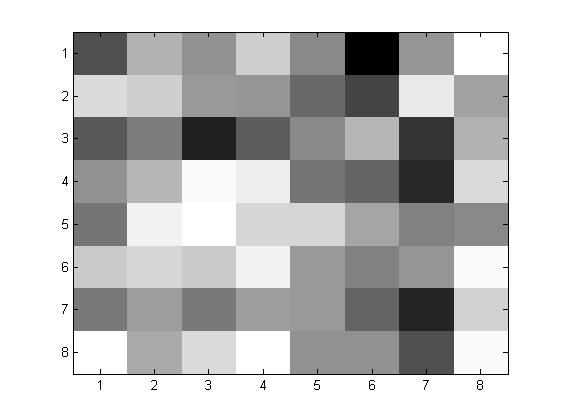
\includegraphics[width=0.7\textwidth]{combinedconfusion.jpg}
	\caption{Waarschijnlijkheids matrix voor de gewogen fingerprints. Op de x as de test locaties en op de y as de train locaties. Hoe lichter de kleur des te groter de waarschijnlijkheid om op die locatie te zijn\\gewicht line = 0.5; gewicht blob = 1}
	\label{fig:combinedconfusion}
\end{figure}
\begin{figure}[h]
	\centering
	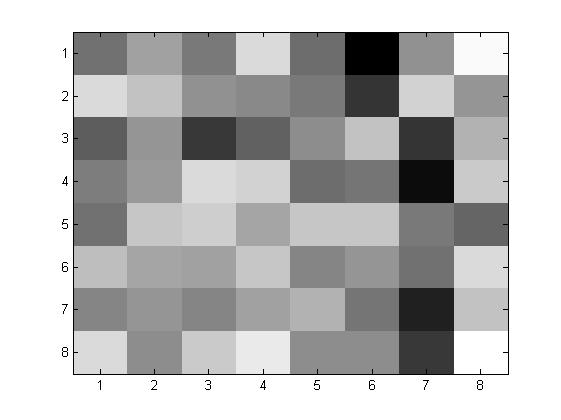
\includegraphics[width=0.7\textwidth]{combinedconfusion_concat.jpg}
	\caption{Waarschijnlijkheids matrix voor de geconcateneerde fingerprints.  Op de x as de test locaties en op de y as de train locaties. Hoe lichter de kleur des te groter de waarschijnlijkheid om op die locatie te zijn}
	\label{fig:combinedconfusion_concat}
\end{figure}
\begin{figure}[h]
	\centering
	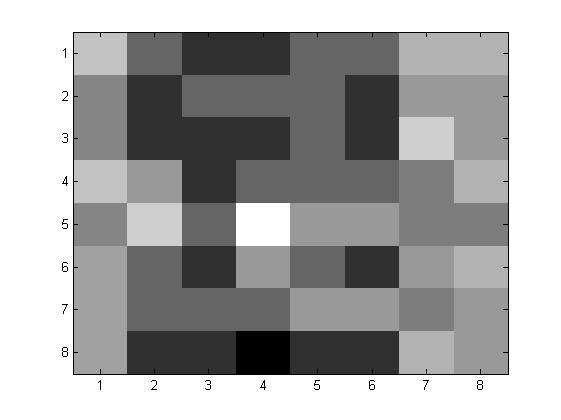
\includegraphics[width=0.7\textwidth]{linelength.jpg}
	\caption{Waarschijnlijkheids matrix voor de line length fingerprint localisatie.}
	\label{fig:linelength}
\end{figure}
\end{document}

